\section{Введение}

Выделяют 3 модели нейронов:

\begin{enumerate}
    \item \textbf{Физиологические} -- нас не интересуют, понять как работает нейрон
    \item \textbf{Феноменологические} -- не рассмтариваем, они для биологов
    \item \textbf{Формальный нейрон} -- будем заниматься ими, математическая модель, попытка ее создать, не отражает работу физического нейрона.
\end{enumerate}

\subsection{Модель МакКалака Питтса}

\begin{equation*}
    y = \phi(\nu) = \frac{1}{1 + e^{-\alpha \nu}}
\end{equation*}

\begin{equation*}
    y = \th(\nu) = \frac{1 - e^{-2\alpha\nu}}{1 + e^{-2\alpha\nu}}
\end{equation*}

\begin{equation*}
    \frac{d \varphi}{d \nu} = \alpha \varphi(\nu)(1 - \varphi(\nu))
\end{equation*}

\begin{equation*}
    \frac{d \varphi}{d \nu} = \alpha (1 - \varphi^2(\nu))
\end{equation*}

\subsubsection{OR}

\begin{center}
\begin{tikzpicture}
  \begin{axis}[
    xlabel=$x_1$,
    ylabel={$x_2$},
    minor tick num = 10,
    domain=-1:1,
    legend pos = north west,
    grid = major,
    line width = 1
  ]
  \legend{
        $x_2 = -x_1 + 0.5$,
        Значения
  }
    \addplot [blue] {-x + 0.5};
    \addplot [only marks] table {
        0 1
        1 0
        0 0
        1 1
    };
  \end{axis}
\end{tikzpicture}
\end{center}

\subsubsection{AND}

\begin{center}
\begin{tikzpicture}
  \begin{axis}[
    xlabel=$x_1$,
    ylabel={$x_2$},
    minor tick num = 10,
    domain=-0.5:1.5,
    legend pos = north west,
    grid = major,
    line width = 1
  ]
  \legend{
        $x_2 = -x_1 + 1.5$,
        Значения
  }
    \addplot [blue] {-x + 1.5};
    \addplot [only marks] table {
        0 1
        1 0
        0 0
        1 1
    };
  \end{axis}
\end{tikzpicture}
\end{center}

\subsubsection{XOR}

\begin{center}
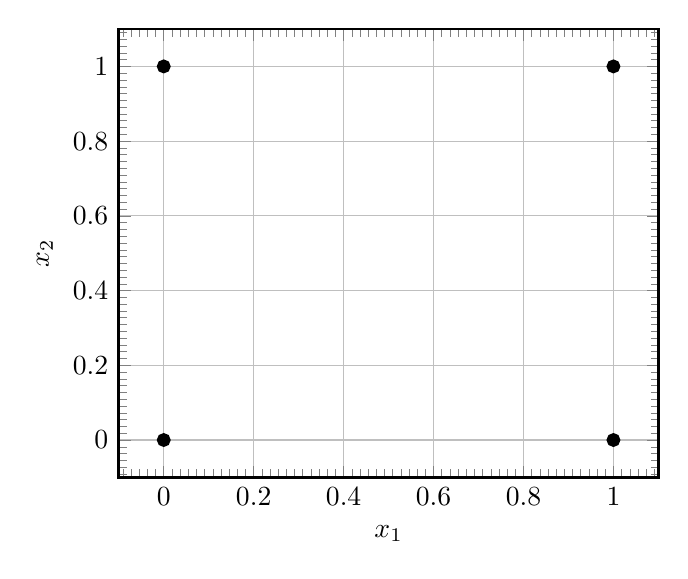
\begin{tikzpicture}
  \begin{axis}[
    xlabel=$x_1$,
    ylabel={$x_2$},
    minor tick num = 10,
    legend pos = north west,
    grid = major,
    line width = 1
  ]
    \addplot [only marks] table {
        0 1
        1 0
        0 0
        1 1
    };
  \end{axis}
\end{tikzpicture}
\end{center}

\subsection{Какие задачи решают нейронные сети}

\begin{itemize}
    \item распознавание (классификация) образов
    \item прогнозирование
    \item аппроксимация функций
    \item фильтрация
    \item ассоциативная память
    \item кластеризация пространства
\end{itemize}

\subsection{Правила Хебба}

\begin{enumerate}
    \item Если два нейрона по обе стороны синапса активизируются одновременно, то прочность этого соединения возрастает;
    \item Если два нейрона по обе стороны синапса активизируются асинхронно, то прочность этого соединения понижается.
\end{enumerate}

\begin{equation*}
    \Delta \omega_{kj} = \eta y_kx_j
\end{equation*}
